\documentclass[12pt]{article}
\usepackage{fullpage}
\usepackage{enumitem}
\usepackage{amsmath}
\usepackage{amssymb}
\usepackage{graphicx}
\usepackage{bm}
\usepackage{hyperref}
\usepackage{bbm}
\usepackage{verbatim}

\begin{document}

\begin{center}
{\Large CS221 Fall 2018 Homework 6}

\begin{tabular}{rl}
SUNet ID: & 05794739 \\
Name: & Luis Perez \\
Collaborators: &
\end{tabular}
\end{center}

By turning in this assignment, I agree by the Stanford honor code and declare
that all of this is my own work.

\section*{Problem 0}

\begin{enumerate}[label=(\alph*)]
  \item Constructing the CSP from this problem statement is somewhat straight-forward. We present the construct CSP below. We assume that each lighbulb is initially off.
  \begin{itemize}
    \item Variables: For each button $j = 1, \cdots, m$, we have a variable $B_i \in \{0,1\}$. We explicitly mention now that the Domain of each variables is $\{0,1\}$. Intuitively, each variable simply represents whether or not button $j$ is pressed.
    \item Constraints: Lightbulbs are on only if toggled an odd number of times by the buttons selected. We set-up $n$ constraints (1-per lightbulb).
    \begin{itemize}
      \item Constraint Scope: For each lightbulb $i$, we define the set $M_i = \{j \mid i \in T_j \}$ (this is the set of buttons that toggle lighbulb $i$) and the scope $\text{Scope}(i) = \{B_k \mid k \in M_i \}$.
      \item Constraint Expression: We then have the constraint expression given by $f_i(\text{Scope}(i)) = \left(\sum_{k} B_k\right) \mod 2$. 
    \end{itemize}
    The above enforce the constraint that for each lighbulb, an odd number of toggles must have been triggered given the configuration (since the lighbulbs start off, and odd number of toggles will leave them in the on position).
  \end{itemize}
  The above Variables and Constraints are sufficient to solve the problem. A solution exists if and only if the weight is $1$. Given our definition of constraints above, this implies that $\forall i$, $f_i(b) = 1$, which means that our selection of touched buttons must lead to all lighbulbs being turned on.

  \item
    \begin{enumerate}[label=\roman*]
      \item There are two consistent assignments. $X_1 = 1, X_2 = 0, X_3 = 1$ and $X_1 = 0, X_1 = 1, X_2 = 0$.
      \item `backtrack' will be called 9 times (including initial call) if we use the fixed ordering specified in the problem statement. The resulting call-stack (in tree form) is presented in Figure \ref{fig:backtrack_simple}.
        \begin{figure}[!h]
          \centering
          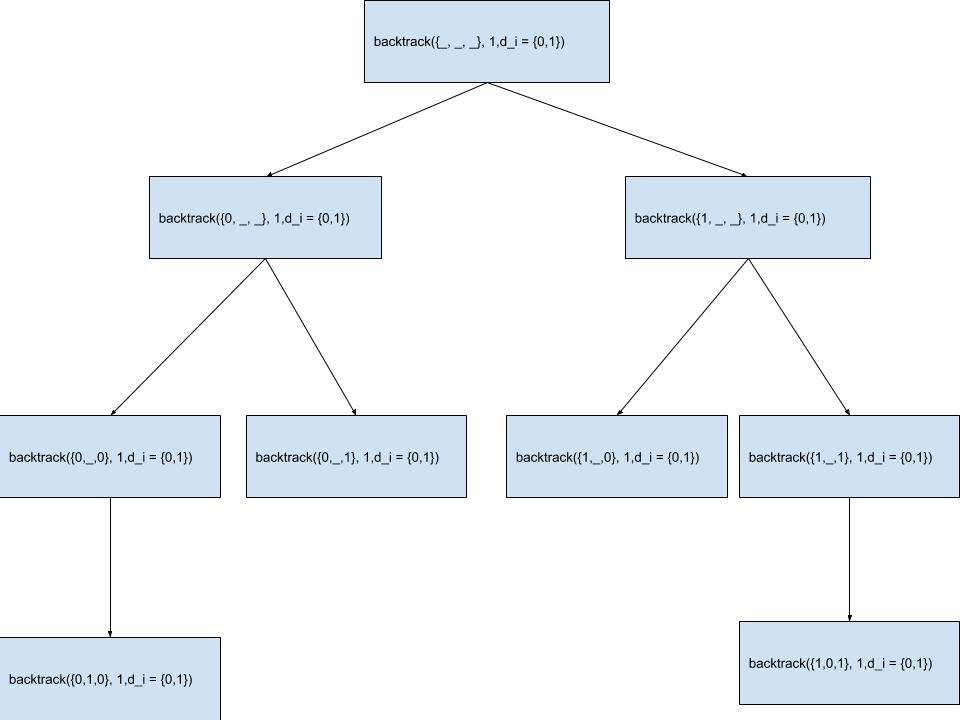
\includegraphics[scale=0.3]{backtrack.jpg}
          \caption{Backtrack using domain ordering ${0,1}$ and variable ordering ${X_1, X_3, X_2}$}
          \label{fig:backtrack_simple}
        \end{figure}
      \item `backtrack' will be called 7 times (including initial call) if we use the fixed ordering specified in the problem statement with AC-3. The resulting call-stack (in tree form) is presented in Figure \ref{fig:backtrack_ac3}.
       \begin{figure}[!h]
          \centering
          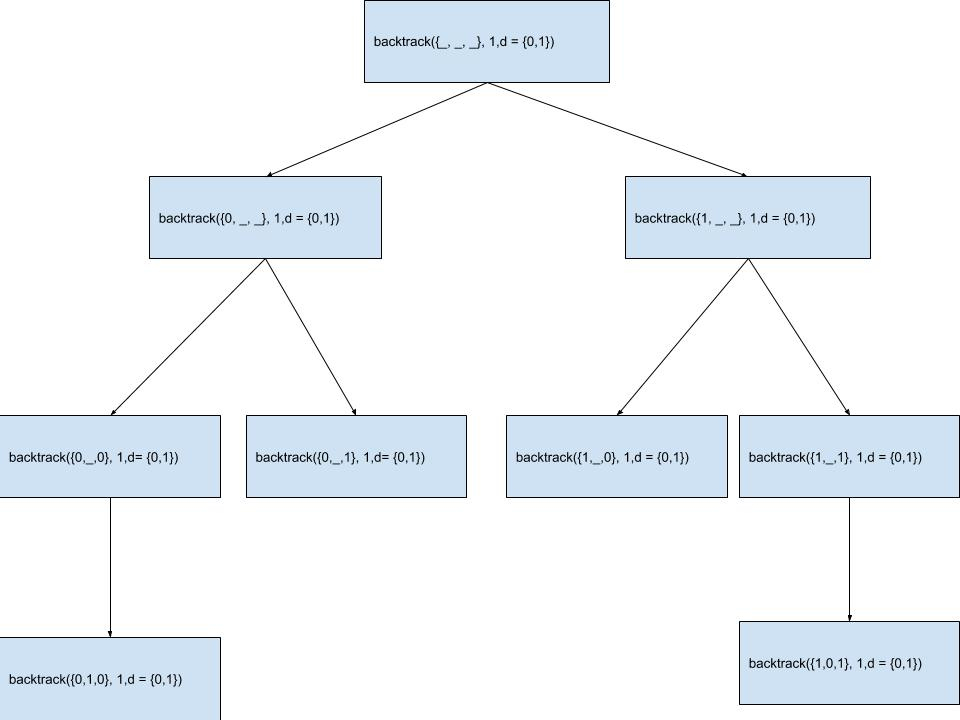
\includegraphics[scale=0.3]{backtrack_ac3.jpg}
          \caption{Backtrack using domain ordering ${0,1}$ and variable ordering ${X_1, X_3, X_2}$ with AC-3}
          \label{fig:backtrack_ac3}
        \end{figure}
    \end{enumerate}
    \item In ``submission.py''.
\end{enumerate}

\section*{Problem 1}

\begin{enumerate}[label=(\alph*)]
  \item In ``submission.py''.
  \item In ``submission.py''.
  \item In ``submission.py''.
\end{enumerate}

\section*{Problem 2}

\begin{enumerate}[label=(\alph*)]
  \item As the hint suggest, we draw inspiration from the lecture slides. We therefore introduce the auxilirary variables $S_i$ for $1 \leq i \leq 3$ consisting of a tuple. The first element of this tuple will be equal the sum  of the elements $X_1, \cdots, X_{i-1}$, and the second element of this tuple will be equal to the sum of variables $X_1, \cdots X_{i}$. For simplicity, we can make all these variables have the same domain which is simply given by: $\{0,1,2,3,4,5,6 \} \times \{0,1,2,3,4,5,6 \}$.

  More generally, the straight-forward domain is given by the below, where we assume that $\forall i, x \in \text{Domain}(X_i), x \geq 0$:
  $$
    \text{Domain}(S_i) = \{0,1, \cdots, m \} \times \{ 0,1,\cdots m \}
  $$
  where $m = \sum_{i=1}^n \max\left\{ \text{Domain}(X_i) \right\}$. A simple modification to restrict our domain a bit further is to make $m$ depend on $i$ such that $m_i = \sum_{j=1}^{i} \max\left\{ \text{Domain}(X_j) \right\}$ and $m_1 = 0$. In that case, or domain is given by:
  $$
    \text{Domain}(S_i) = \{0,1,\cdots, m_{i-1} \} \times \{0, 1, \cdots m_i \}
  $$
  If we care to, we can restrict the domain even further, to the below:
  \begin{align*}
   \text{Domain}(S_1) &= \{0 \} \times \{\text{Domain}(X_1) \} \\
   \text{Domain}(S_i) &=  \{ (s_1,s_2) \mid (\_, s_1) \in \text{Domain}(S_{i-1}), s_2 \in \{ s_1 + v \mid v \in \text{Domain}(X_i) \} \}
  \end{align*}
  Regardless of which domain we pick, we now describe the factors that we must introduce.
  \begin{itemize}
    \item Initializations: $\mathbbm{1}[S_1[1] = 0]$. This enforces that we start our sum at $0$.
    \item Processing: $\forall i, \mathbbm{1}[S_i[2] = S_i[1] + X_i]$. This enforces that we are computing the sum.
    \item Final outputs: $\mathbbm{1}[S_n[2] \leq k]$. This is enforcing our initial constraint from the problem that the sum must be less than our equal to $k$.
    \item Consistency: $\forall i, \mathbbm{1}[B_{i}[1] = B_{i-1}[2]]$. This enforces that our computed sums are transferred correctly between tuples.
  \end{itemize}
  The above constraints, along with a concrete example, can the nicely summarized in Figure \ref{fig:n-ary}. It is clear that the above scheme will work, assigning only valid values to $X_i$.
  \begin{figure}[!h]
    \centering
    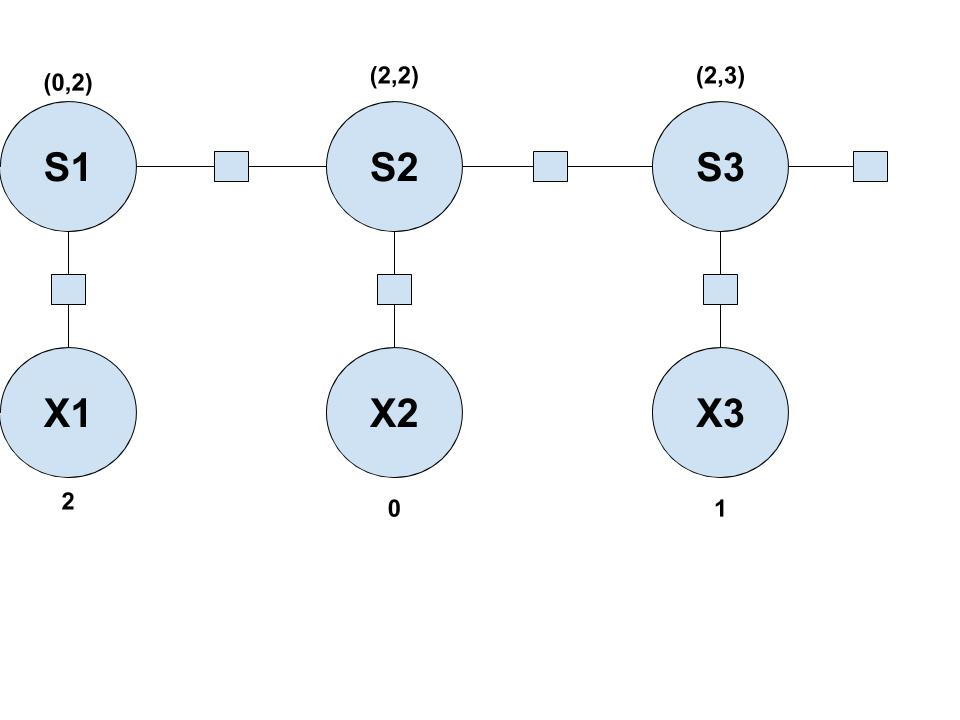
\includegraphics[scale=0.2]{n-ary.jpg}
    \caption{Reducing $n-ary$ constraint to binary and unary constraints.}
    \label{fig:n-ary}
  \end{figure}

  \item In ``submission.py''.
\end{enumerate}

\section*{Problem 2}

\begin{enumerate}[label=(\alph*)]
\item In ``submission.py''.
\item In ``submission.py''.
\item I set up my profile as per below. It didn't work out very well. A few classes are incorrect (CS224N is offered in Winter, for example, not just Autumn), and it was not good at long-term planning for part-time students (like myself). It would also be nice to specify all undergraudate courses in a field as pre-satisfied, rather than having to list them out. The next good feature would be the ability to request the same course under multiple requests.

\begin{verbatim}
Here's the best schedule:
Quarter   Units Course
  Spr2019 3 CS166
  Win2019 3 CS154
\end{verbatim}

\begin{verbatim}
minUnits 0
maxUnits 4

# These are the quarters that I need to fill out.
# It is assumed that the quarters are sorted in chronological order.
register Spr2019
register Sum2019
register Aut2019
register Win2019
register Spr2020
register Sum2020

# Courses I've already taken
taken CS103
taken CS109
taken CS161
taken CS107
taken CS110
taken STATS237
taken CS228
taken CS224W
taken CS155
taken CS221
taken CS106A
taken CS106B
taken CS124
taken CS145
taken CS157
taken EE102A
taken EE178
taken EE278A
taken ENGR105
taken LINGUIST130A
taken LINGUIST180
taken MATH113
taken MATH115
taken MATH51
taken PHIL150
taken STATS116
taken STATS305
taken CS224N

# Courses that I'm requesting
request CS205A or CS225A or CS227B or CS229T or CS231B or CS232 or CS270 or CS273A or CS274 or CS275 or CS276 or CS331A or CS331B or CS371 or APPPHYS293 or BIOE332 or EE263 or EE364B or EE376A or ENGR205 or ENGR209A or MS&E251 or MS&E252 or MS&E351 or MS&E352 or MS&E353 or STATS202 or STATS315A or STATS315B or CS223A or CS224S or CS229 or CS224U or CS231A
request CS154
request CS246 or CS261 or CS265 or CS268 or CS354 or CS362 or CS367
request CS166
request CS254 or CS262 or CS266 or CS334A or CS355 or CS364A or CS374
request CS228 or CS255 or CS263 or CS267 or CS341 or CS357 or CS366 or EE364A


\end{verbatim}
\end{enumerate}

\end{document}